
% tex-thesis.tex
% Latex Beispiel-Dokument zur Erstellung einer Abschluss- oder Projektarbeit
% Hochschule Emden/Leer | C.Koch | 4. September 2011

\documentclass[twoside,a4paper,11pt]{book}
%
\usepackage[ngerman]{babel} 	% german language support
\usepackage[T1]{fontenc}    	% german language support
\usepackage[utf8]{inputenc}	% character coding of input files
%
% load special packages to extend the basic LaTeX features
\usepackage[dvips]{graphicx}    % enable EPS picture import
\usepackage{calc}               % improvement of std. calculation features \emph{i.e.} length
\usepackage{makeidx}            % enable indexing
\usepackage{color}              % for creating colored boxes, i.e. for psfrag replacements
\usepackage{lscape}             % rotate some figures and tables 90 Deg onto a new page
\usepackage[hang,small,scriptsize,bf]{caption} % resize the figure label
\usepackage{amssymb}            % for special math symbols
\usepackage{nomencl}            % for nomenclature (list of abbreviations)
\usepackage[tight]{minitoc}     % create a small table of contense for each chapter
\usepackage{sectsty}            % section headings in helvetica
\allsectionsfont{\sffamily}

\usepackage{hsel-thesis2011}    % ParStart etc.

%
\pagestyle{headings}           % use default headers and footers
%*************************************************
%
%       Headerstyle
%       C.Koch
%       file for determining the general footers
%       and headers of this document
%       Created 21.02.2001
%
%*************************************************


% tune page headers and footers
% for details see manual of fancyhdr
\usepackage{fancyhdr}
\pagestyle{fancy}

% defining the layout for common pages
\fancyhead{}                    % clear all fields  ... header
\fancyfoot{}                    %   -'-             ... footer

% re-defining \rightmark and \leftmark
\renewcommand{\chaptermark}[1]{%
 \markboth{\chaptername \ \thechapter.\ #1}{}}
\renewcommand{\sectionmark}[1]{\markright{\thesection.\ #1}{}}

\fancyhead[RO,LE]{\thepage}     % print page number on every page
\fancyhead[LO]{\rightmark}      % odd pages: chapter information
\fancyhead[RE]{\leftmark}       % even pages: section information

% draw a thin line across the page
\renewcommand{\headrulewidth}{0.4pt}

% defining the layout for pages which switch automatically to 'plain' (CHAPTERS, etc.)
\fancypagestyle{plain}{%
\fancyhf{} % clear all header and footer fields
\fancyhead[RO,LE]{\thepage}     % print page number
%\fancyhead[L]{\thepage} % except the left corner
\renewcommand{\headrulewidth}{0.4pt}
\renewcommand{\footrulewidth}{0pt}}
             % use fancy headers
%
\makeindex                      % generate sorted index file
\makeglossary                   % syntax for generating nomenclature file: makeindex 'filename.glo' -s nomencl.ist -o 'filename.gls'

%
% use this command to compile only ONE chapter/file
%\includeonly{introduction}
%
\begin{document}
%
\bibliographystyle{plain}
%
\dominitoc[n]               % generate minitocs for every chapter
\pagenumbering{Roman}       % set page numbers to roman style

\begin{titlepage}
	
	\vspace{-0.5cm}
	\hspace{-2.0cm}
	\begin{tabular}{p{8.0cm} p{8.0cm}}
		
\includegraphics[width = 6.0cm]{img/hsel-allgemein} &
		\parbox[b]{8.0cm}{
			{\large 	Fachbereich Technik }\\
			{\large 	Abteilung Elektrotechnik und Informatik }     
		} \\
		\\
		\hline
	\end{tabular}
	%
	\begin{center}
		
		\vspace{2.5cm}%
		\LARGE{\textsc{ %
			ARM WHITEPAPER}}\\
		
		\vspace{1cm}%
		\LARGE{\textsc{	CACHE SPECULATION SIDE-CHANNELS}}\\
		
		\vspace{2.0cm}%
		\LARGE{\textsc{%
				{PROJEKTARBEIT} % ODER: Projektarbeit
		}}\\
		%\large
		%zur Erlangung des akademischen Grades % ODER: Studiengang Informatik
		
		\vspace{2cm}%
		\large
		Vorgelegt von\\ Xingjian Chen\\ Studiengang Informatik\\ 7007806 
		
		\vspace{1cm} 
		Emden, \today
		
		\vspace{2.5cm}%
		Betreut von\\ Prof. Dr.-Ing. Gerd von Cölln
		
	\end{center}
	\normalsize
\end{titlepage}             % title page with subject and print date
\linespread{1.2}            % line spacing factor -> causes trouble with minitoc!
\noitemsep
%
%\setcounter{page}{6}   % modify start value (for book-version only)
%
\chapter*{Rechtliche Erklärung}
\label{sec:Declaration} %
\addcontentsline{toc}{section}{Rechtliche Erklärung}
%
\vspace{1.5cm}
\begin{itemize}
\item[ {\bf [~~]} ] Die vorliegende Arbeit entstand in Zusammenarbeit mit einer In\-sti\-tution, Firma oder Person außerhalb der Hochschule Emden/Leer.

\item[ {\bf [~~]} ] Die vorliegende Arbeit enthält vertrauliche oder kommerziell nutzbare Informationen, deren Rechte außerhalb der Hochschule Emden/Leer liegen. Sie darf nur den am Prüfungs\-verfahren beteiligten Personen zugänglich gemacht werden, die hiermit auf ihre Pflicht zur Vertraulichkeit hingewiesen werden.

\item[ {\bf [~~]} ] Soweit meine Rechte berührt sind, erkläre ich mich einverstanden, dass die Bachelor-Arbeit Angehörigen der Hochschule Emden/Leer für Studium, Lehre und Forschung uneingeschränkt zugänglich gemacht werden kann. 

\end{itemize}
%
\vspace{2.0cm}

Hiermit erkläre ich an Eides statt, dass ich die vorliegende Arbeit bis auf die offizielle Betreuung selbst und ohne fremde Hilfe angefertigt habe und die benutzten Quellen und Hilfsmittel vollständig angegeben sind.

\vspace{2.0cm}

\begin{tabular}{p{5.0cm}}
   \hline
   Datum, Unterschrift
\end{tabular}

%*************************************************
%
%       Lists
%       C.Koch
%       Created 02.02.2001
%
%*************************************************

\tableofcontents
%\addcontentsline{toc}{section}{List of Figures}%
\listoffigures %
%\addcontentsline{toc}{section}{List of Tables}%
\listoftables
%
\cleardoublepage
\addcontentsline{toc}{section}{\nomname}%
%\linespread{0.6} %  default line spread
\printnomenclature%
%\linespread{1.2} % current line spread
%
\newpage

%
\chapter*{Danksagung}
\label{sec:Ack}%
% add this page manually to the table of contents with ROMAN letters
\addcontentsline{toc}{section}{Danksagung}
%
The author would like to thank Prof.~T.J.~Ellis and
Prof.~A.~Georgiadis for their supervision, encouragement and
valuable discussions. The author is also very grateful to
Dipl.-Ing.~J.~Mahalek who triggered this very interesting project
and to Dipl.-Ing.~L.~Eisenmann for fruitful discussions and
contributions in the development of systems for detecting
occupants and for his support at BMW.\\

I wish to thank Dr.~S-B.~Park for his introduction to CMOS cameras
and smart illumination and his tireless explanations. I will never
forget our in-circuit software development during high-speed test
drives. I also have to thank J.J.~Yoon for his support in multiple
mathematical problems and value discussions about illumination
strategies.

Special thanks to my fellows at BMW who helped me bring our
HDR-camera from illusions and raw ideas to reality: S.~Akisogulu,
W.~Solka, S.~Weidhaas and A.~Augst. I also express my gratitude to
the fellows who looked carefully through this manuscript and
helped to improve it with a number of corrections, suggestions and
good
questions.\\

Finally I want to thank my wonderful wife Melanie
for her constant faith, love and encouragement.\\
%
\vspace{4.0cm}
%
\begin{center}
The majority of this research was sponsored by
BMW\index{BMW}\nomenclature{BMW}{Bayerische Motorenwerke} and
performed at the BMW AG Research and Innovation Center in Munich,
Germany. The opinions expressed herein are those of the author and
do not
necessarily represent those of BMW. %\vspace{0.5cm}
\end{center}

\section{Kurzfassung}
text

\noindent
text

%
\cleardoublepage            % for correct page numbering / margin
\pagenumbering{arabic}      % reset page numbers to arabic style
%

\chapter{Einleitung}

\section{Motivation}

Die Bachelor- oder Masterarbeit ist ein besonders wichtiger Bestandteil des Studiums in den Abschlusssemestern. Sie stellt
eines der wenigen gegenständlich vorzeigbaren Arbeitsergebnisse des Studiums dar und ist auch deshalb, z.B.
bei Bewerbungen, von besonderer Bedeutung. Es liegt daher im Interesse eines jeden Studierenden, eine
sowohl inhaltlich als auch vom äußeren Erscheinungsbild her hohen Ansprüchen gerecht werdende
Dokumentation der Abschlussarbeit zu erstellen. Die nachfolgenden Hinweise sollen dabei Hilfestellung bieten.\\

Gegenstand des einleitenden Kapitels ist es, dem Leser einen Überblick über für die Arbeit relevante Grundlagen und verwandten Arbeiten zu geben. Folgende grundlegende Fragen sollten beantwortet werden:
\begin{itemize}
	\item Warum wird das Thema der Arbeit behandelt? 
	\item Wie lautet die genaue Aufgabendefinition?
	\item Welche Fragenstellungen werden in der Arbeit behandelt?	
	\item Wie ist die Arbeit strukturiert?  
\end{itemize}

Das Kapitel zur Einleitung dient dem Leser vorrangig als Entscheidungshilfe: Ist die Arbeit für mich überhaupt relevant? Werden für mich interessante Fragestellungen in der Arbeit behandelt? Sofern den Leser nur Teilergebnisse interessieren: Wo finde ich diese?

Die Motivation zur Projektarbeit kann vielfältig sein und sollte daher ausreichend begründet werden. Beispiele: Ein bestehendes Problem wurde durch den Stand der Technik bisher nicht oder nicht zufriedenstellend gelöst. Oder: Gegenstand der Arbeit ist eine besonders kostengünstige Lösung. Oder auch: Die Arbeit behandelt eine grundlegende Evaluation, um Möglichkeiten als auch Limitationen einer neuen Technologie aufzuzeigen.

Um dem Leser den logischen Aufbau und die Zusammenhänge einzelner Kapitel zu verdeutlichen ("roter Faden"), bieten sich beispielsweise Formulierungen an wie "Nachdem im zweiten Kapitel die Grundlagen der BlueTooth-Technologie behandelt wurde, wird im Kapitel 3 die Realisierung eines Systems zur Ortung von Satelliten mittels BlueTooth beschrieben. Anschließend folgt die Auswertung der in Kapitel 4 definierten Experimente zur Performanz des Systems".

\section{Formalien}

Dieser Abschnitt \dots

\section{Beispiel}

Dieser Abschnitt beinhaltet einen Ausschnitt aus der Ballade ''Erlkönig'' von Johann Wolfgang von Goethe~\cite{Goethe1782}.


{\it ''Wer reitet so spät durch Nacht und Wind? Es ist der Vater mit seinem Kind.
Er hat den Knaben wohl in dem Arm, Er faßt ihn sicher, er hält ihn warm.

Mein Sohn, was birgst du so bang dein Gesicht?
Siehst Vater, du den Erlkönig nicht!
Den Erlenkönig mit Kron' und Schweif?
Mein Sohn, es ist ein Nebelstreif.

Du liebes Kind, komm geh' mit mir!
Gar schöne Spiele, spiel ich mit dir,
Manch bunte Blumen sind an dem Strand,
Meine Mutter hat manch gülden Gewand.

Mein Vater, mein Vater, und hörest du nicht,
Was Erlenkönig mir leise verspricht?
Sei ruhig, bleibe ruhig, mein Kind,
In dürren Blättern säuselt der Wind.

Willst feiner Knabe du mit mir geh'n?
Meine Töchter sollen dich warten schön,
Meine Töchter führen den nächtlichen Reihn
Und wiegen und tanzen und singen dich ein.''
\dots
}

		% example contents

\chapter{Grundlagen und Stand der Technik}

\section{Motivation}
Gegenstand dieses Kapitels ist es, dem Leser einen Überblick über für die Arbeit relevante Grundlagen und verwandten Arbeiten zu geben. Folgende grundlegende Fragen sollten beantwortet werden:
\begin{itemize}
	\item Welche artverwandten Projektarbeiten oder Produkte existieren?
	\item Wo ist der Mangel zum Stand der Technik? Warum ist es notwendig oder relevant, das Thema in der Projektarbeit zu behandeln? 
	\item Wie grenzt sich der grundlegende Lösungsansatz vom Stand der Technik ab?
	\item Existieren Vorarbeiten, auf denen aufgebaut wird?
\end{itemize}

Die Motivation zur Projektarbeit kann vielfältig sein und sollte daher ausreichend begründet werden. Beispiele: Ein bestehendes Problem wurde durch den Stand der Technik bisher nicht oder nicht zufriedenstellend gelöst. Oder: Gegenstand der Arbeit ist eine besonders kostengünstige Lösung. Oder auch: Die Arbeit behandelt eine grundlegende Evaluation, um Möglichkeiten als auch Limitationen einer neuen Technologie aufzuzeigen.

\section{Stand der Technik}

Zum Stand der Technik oder Stand des Wissens gehören alle 

Als Startpunkt für einen ersten Überblick bietet sich die Internet-Suchmaschine Ihres Vertrauens an. Die Qualität der Ergebnisse hängt hierbei grundlegend von den verwendeten Schlüsselwörtern ab. 

Der erste Überblick hilft, weitere relevante Schlüsselwörter zu definieren. Mit diesen bietet sich eine gezieltere Suche in fachspezifischen Datenbanken an. Beispiele:

\begin{itemize}
\item IEEE Explore
\item CiteSeer http://citeseer.ist.psu.edu
\item arXiv http://arxiv.org
\item Google Schoolar
\item ...
\end{itemize}

Innerhalb der Hochschule verfügen Sie über einen kostenfreien Zugang zu Publikationen der IEEE - nutzen Sie diese qualitativ hochwertige Quelle! 

Bitte verwenden Sie zur Darlegung des Stands der Technik vorrangig {\emph nicht flüchtige Quellen}, beispielsweise Publikationen in Form von Buch-, Zeitungs-, oder Konferenzbeiträgen.
Vermeiden Sie nach Möglichkeit {\emph flüchtige Quellen}, beispielsweise Informationen, die ausschließlich durch Internetseiten, Blog-Einträge und dergleichen belegt sind. Der Leser muss die Möglichkeit haben, Ihre durch Literaturangaben hinterfütterten Aussagen noch nach Jahren nachvollziehen zu können - dies ist durch reiche Verwendung sekündlich veränderbarer Inhalte einzelner Internetseiten nicht gegeben.


\chapter{Umsetzung}

\section{Motivation}

Dies Kapitel \dots

\chapter{Bewertung der Ergebnisse}

Dies Kapitel \dots



\chapter{Zusammenfassung und Ausblick}

In diesem Kapitel wird ein Resume zu den Ergebnissen der Arbeit gegeben.
Hierbei ist eine selbstkritische Darstellung angebracht. Was funktioniert? Wie gut funktioniert es: Wie kann die Performanz des Systems numerisch beschreiben werden? Konnte die Aufgabenstellung vollständig umgesetzt werden? Was funktioniert nicht? 
Beispiel: ''Das realisierte Kamerasystem ist in der Lage, bis zu 90 Bilder in der Sekunde aufzunehmen, siehe Kapitel. Dies geht signifikant über die in der Aufgabenstellung geforderten 60 Bilder pro Sekunde hinaus. Aufgrund der limitierten Bandbreite des CAN-Bus, ist das Kamerasystem jedoch ohne Bildkompression lediglich in der Lage, 50 Bilder pro Sekunde an einen PC zu übertragen''.

Insbesondere die Abgrenzung zu Themen, die explizit nicht behandelt wurden, sollten hervorgehoben werden und dienen als Vorlage für den Ausblick auf Folgearbeiten. Beispiel: ''Die Realisierung einer Bildkompression als auch eine deutliche Reduzierung des Energieverbrauchs, ist Gegenstand weiterführender Arbeiten.''


\bibliography{myliterature}
%
\appendix
%

\chapter{Einen hab ich noch}

\section{Weiterführende Erläuterungen}

Inhalte, die nicht im direkten Fokus der Aufgabenstellung stehen, jedoch zur Ausarbeitung indirekt beigetragen haben oder zum besseren Verständnis der dargestellten Aussagen beitragen, finden im Anhang der Arbeit eine passende Position.

\section{Messdaten}

Im begrenzten Umfang ist es auch hilfreich, weiteres Datenmaterial der Arbeit hinzuzufügen, beispielsweise Tabellen, Messreihen, kleinere Skripte, etc.



%% tex-thesis.tex
% Latex Beispiel-Dokument zur Erstellung einer Abschluss- oder Projektarbeit
% Hochschule Emden/Leer | Eugen Betuch | 2016

\documentclass[a4paper,11pt, oneside]{article}
%
\usepackage[ngerman]{babel} 	% german language support
\usepackage[T1]{fontenc}    	% german language support
\usepackage[utf8]{inputenc}	% character coding of input files
		
\usepackage[cmex10]{amsmath}
%
% load special packages to extend the basic LaTeX features
\usepackage[dvips]{graphicx}    % enable EPS picture import
\usepackage{calc}               % improvement of std. calculation features \emph{i.e.} length
\usepackage{color}              % for creating colored boxes, i.e. for psfrag replacements
\usepackage{lscape}             % rotate some figures and tables 90 Deg onto a new page
\usepackage[hang,small,scriptsize,bf]{caption} % resize the figure label
\usepackage{amssymb}            % for special math symbols
%\usepackage[tight]{minitoc}     % create a small table of contense for each chapter
\usepackage{sectsty}            % section headings in helvetica
\usepackage{eurosym}
\usepackage{url}
\usepackage{natbib}
\usepackage{xcolor}
\usepackage{float}
\usepackage{subfig}
\usepackage{tabularx}
\usepackage{setspace}
\usepackage{lmodern}
\usepackage{inconsolata}


\usepackage{color}

\definecolor{ppurple}{rgb}{0.5,0,0.35}
\definecolor{pgreen}{rgb}{0,0.5,0}
\definecolor{pred}{rgb}{0.9,0,0}
\definecolor{pgrey}{rgb}{0.46,0.45,0.48}

\usepackage{listings}
\usepackage{textcomp}
\lstset{ %
	language=C++,                % choose the language of the code
	basicstyle=\footnotesize,       % the size of the fonts that are used for the code
	keywordstyle=\color{ppurple}\ttfamily,
	stringstyle=\color{pred}\ttfamily,
	commentstyle=\bfseries\color{pgreen},
	numbers=left,                   % where to put the line-numbers
	numberstyle=\footnotesize,      % the size of the fonts that are used for the line-numbers
	stepnumber=1,                   % the step between two line-numbers. If it is 1 each line will be numbered
	numbersep=5pt,                  % how far the line-numbers are from the code
	backgroundcolor=\color{white},  % choose the background color. You must add \usepackage{color}
	showspaces=false,               % show spaces adding particular underscores
	showstringspaces=false,         % underline spaces within strings
	showtabs=false,                 % show tabs within strings adding particular underscores
	frame=single,           % adds a frame around the code
	tabsize=2,          % sets default tabsize to 2 spaces
	captionpos=b,           % sets the caption-position to bottom
	breaklines=true,        % sets automatic line breaking
	breakatwhitespace=false,    % sets if automatic breaks should only happen at whitespace
	escapeinside={\%*}{*)}          % if you want to add a comment within your code
}

\usepackage[section]{placeins} % force figures in their sections

\hyphenation{OSI-Referenz-modells}

\allsectionsfont{\sffamily}

\usepackage{hsel-thesis2011}    % ParStart etc.
\usepackage{booktabs}

%
\pagestyle{headings}           % use default headers and footers
%*************************************************
%
%       Headerstyle
%       C.Koch
%       file for determining the general footers
%       and headers of this document
%       Created 21.02.2001
%
%*************************************************


% tune page headers and footers
% for details see manual of fancyhdr
\usepackage{fancyhdr}
\pagestyle{fancy}

% defining the layout for common pages
\fancyhead{}                    % clear all fields  ... header
\fancyfoot{}                    %   -'-             ... footer

% re-defining \rightmark and \leftmark
\renewcommand{\chaptermark}[1]{%
 \markboth{\chaptername \ \thechapter.\ #1}{}}
\renewcommand{\sectionmark}[1]{\markright{\thesection.\ #1}{}}

\fancyhead[RO,LE]{\thepage}     % print page number on every page
\fancyhead[LO]{\rightmark}      % odd pages: chapter information
\fancyhead[RE]{\leftmark}       % even pages: section information

% draw a thin line across the page
\renewcommand{\headrulewidth}{0.4pt}

% defining the layout for pages which switch automatically to 'plain' (CHAPTERS, etc.)
\fancypagestyle{plain}{%
\fancyhf{} % clear all header and footer fields
\fancyhead[RO,LE]{\thepage}     % print page number
%\fancyhead[L]{\thepage} % except the left corner
\renewcommand{\headrulewidth}{0.4pt}
\renewcommand{\footrulewidth}{0pt}}
             % use fancy headers
%
%\makeindex                      % generate sorted index file
%\makeglossary                   % syntax for generating nomenclature file: makeindex 'filename.glo' -s nomencl.ist -o 'filename.gls'

%
% use this command to compile only ONE chapter/file
%\includeonly{introduction}
%
\begin{document}
%
%\bibliographystyle{plain}
%
%\dominitoc[n]               % generate minitocs for every chapter
\pagenumbering{Roman}       % set page numbers to roman style

\begin{titlepage}
	
	\vspace{-0.5cm}
	\hspace{-2.0cm}
	\begin{tabular}{p{8.0cm} p{8.0cm}}
		
\includegraphics[width = 6.0cm]{img/hsel-allgemein} &
		\parbox[b]{8.0cm}{
			{\large 	Fachbereich Technik }\\
			{\large 	Abteilung Elektrotechnik und Informatik }     
		} \\
		\\
		\hline
	\end{tabular}
	%
	\begin{center}
		
		\vspace{2.5cm}%
		\LARGE{\textsc{ %
			ARM WHITEPAPER}}\\
		
		\vspace{1cm}%
		\LARGE{\textsc{	CACHE SPECULATION SIDE-CHANNELS}}\\
		
		\vspace{2.0cm}%
		\LARGE{\textsc{%
				{PROJEKTARBEIT} % ODER: Projektarbeit
		}}\\
		%\large
		%zur Erlangung des akademischen Grades % ODER: Studiengang Informatik
		
		\vspace{2cm}%
		\large
		Vorgelegt von\\ Xingjian Chen\\ Studiengang Informatik\\ 7007806 
		
		\vspace{1cm} 
		Emden, \today
		
		\vspace{2.5cm}%
		Betreut von\\ Prof. Dr.-Ing. Gerd von Cölln
		
	\end{center}
	\normalsize
\end{titlepage}             % title page with subject and print date
%\cleardoublepage
%\linespread{1.2}            % line spacing factor -> causes trouble with minitoc!
\noitemsep
%
%*************************************************
%
%       Lists
%       
%       Inhaltsverzeichnis
%
%*************************************************
\tableofcontents
%\addcontentsline{toc}{section}{List of Figures}%
\listoffigures %
%\addcontentsline{toc}{section}{List of Tables}%
%listoftables
%
\cleardoublepage

\newpage 					%enthaelt Inhaltsverzeichis
\cleardoublepage            % for correct page numbering / margin

\pagenumbering{arabic}      % reset page numbers to arabic style

\onehalfspacing
%\let\clearpage\relax		%verhindert Pagebreaks nach includes
\section{Kurzfassung}
text

\noindent
text
		% example contents
%\cleardoublepage
\section{Auswahl der Algorithmen}

Es gibt vier unterschiedlichen Algorithmen auszuwählen.
\begin{enumerate}
	\item Linear Least Square
	\item Least Median Square 
	\item Residual Weighting Algorithm
	\item Non-Linear Least Square
\end{enumerate} 

In dieser Projektarbeit werden Linear Least Square und Least Median Square verwendet. Mittels Linear Least Square kann die gesuchte Position gerechnet werden, aber die Tatsache ist es, dass die fehlerbehaftete Distanzmessungen wegen Non Line of Sight (NLOS)-Verbindung immer vorhanden sind. Deswegen haben berechnete Ergebnisse keine Genauigkeit. Um die optimierte Position zu finden, muss die fehlerbehaftete Distanzmessungen gefiltert werden. Dafür spielt Medien Least Square wichtige Rolle.

Um die beide Algorithmen besser zu verstehen, wird die Lokalisierung eines Sensors unter mathematischen Aspekten betrachtet. Im dreidimensionalen Raum befinden sich N Referenzpunkte (bekannte Sensoren) und ein gesuchter Punkt (unbekannter Sensor). P\textsubscript{1} bis P\textsubscript{N} sind die Referenzpunkte mit den Koordinaten (X\textsubscript{1}, Y\textsubscript{1}, Z\textsubscript{1}) bis (X\textsubscript{N}, Y\textsubscript{N}, Z\textsubscript{N}). P\textsubscript{lat} ist der gesuchte Punkt (X, Y, Z) und R\textsubscript{i} ist die gemessene Distanz von P\textsubscript{lat} zum Referenzpunkt P\textsubscript{i}. In mathematischen Aspekt ist P\textsubscript{lat} tatsächlich ein Schnittpunkt, in dem sich verschiedene Kugeln mit unterschiedlichen Radien im dreidimensionalen Raum überschneiden (vgl. Abb.1). 

\begin{figure}[H]
	\centering
	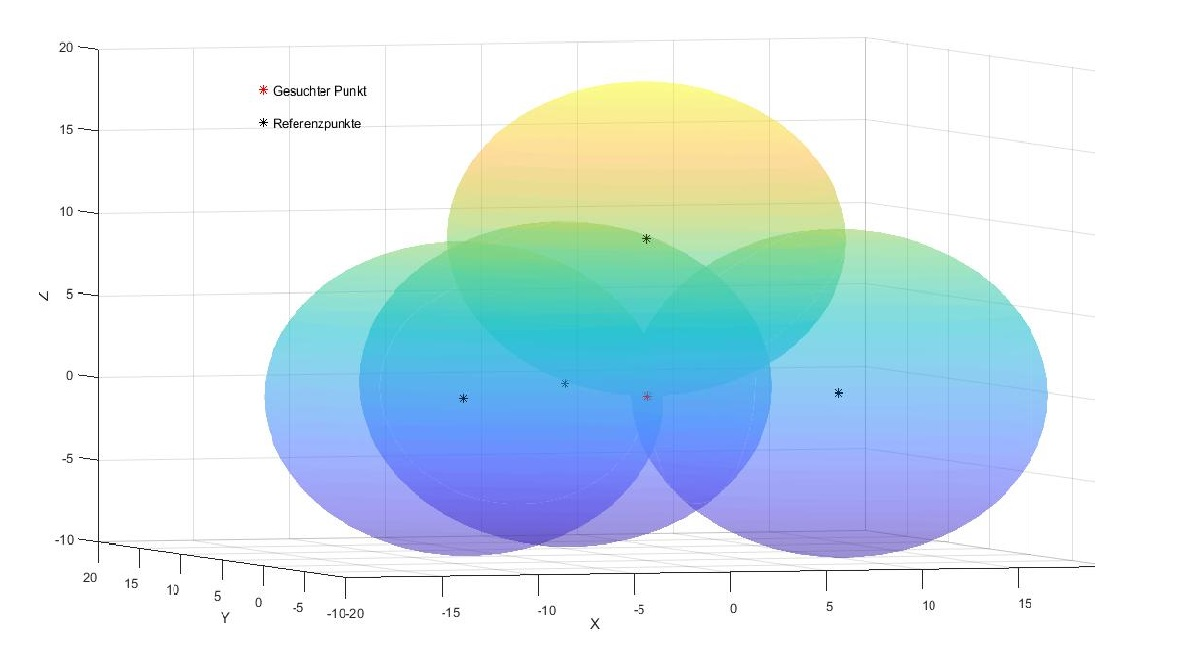
\includegraphics[scale=0.36]{img/Schnittpunkt_3D.jpg}
	\caption{Schnittpunkt verschiedenen Kugeln in einer 3D-Umgebung}
\end{figure}


%\cleardoublepage
\section{Mathematische Ausführung}

\subsection{Aufbau Lineares Gleichungssystems}
Der Aufbau eines linearen Gleichungssystem ist die Voraussetzung, um die gesuchte Position mittels Linear Least Square und Least Median Square zu bestimmen. Die geometrischen Zusammenhänge werden in ein lineares Gleichungssystem wie folgt ausgeführt.
\begin{align}
\underline{A} \cdot \vec{x}= \vec{b}
\end{align}
\newline
Im dreidimensionalen Raum wird die Beziehung zwischen der gesuchte Position P\textsubscript{lat} und P\textsubscript{i}  wie folgt aufgebaut.
\begin{align}
R^{2}_{i}=(X{i}-X)^{2}+(Y{i}-Y)^{2}+(Z{i}-Z)^{2},\quad i \in \mathbb{N}\quad i \ge 4
\end{align}
\newline
Gleichung (2) wird wie folgt umgeformt.
\[
R^{2}_{i} - X^{2}_{i} - Y^{2}_{i} - Z^{2}_{i} = 
(X^{2} + Y^{2} + Z^{2}) - 2 \cdot X{i}\cdot X -2 \cdot Y{i}\cdot Y-2 \cdot Z{i}\cdot Z
\]
\newline
Hier sind fünf Referenzpunkte gegeben. Die Gleichungen können wie folgt aufgestellt werden. 
\[
\begin{split}
R^{2}_{1} - X^{2}_{1} - Y^{2}_{1} - Z^{2}_{1} = 
(X^{2} + Y^{2} + Z^{2}) - 2 \cdot X_{1}\cdot X -2 \cdot Y_{1}\cdot Y-2 \cdot Z_{1}\cdot Z\\
R^{2}_{2} - X^{2}_{2} - Y^{2}_{2} - Z^{2}_{2} = 
(X^{2} + Y^{2} + Z^{2}) - 2 \cdot X_{2}\cdot X -2 \cdot Y_{2}\cdot Y-2 \cdot Z_{2}\cdot Z\\
R^{2}_{3} - X^{2}_{3} - Y^{2}_{3} - Z^{2}_{3} = 
(X^{2} + Y^{2} + Z^{2}) - 2 \cdot X_{3}\cdot X -2 \cdot Y_{3}\cdot Y-2 \cdot Z_{3}\cdot Z\\
R^{2}_{4} - X^{2}_{4} - Y^{2}_{4} - Z^{2}_{4} = 
(X^{2} + Y^{2} + Z^{2}) - 2 \cdot X_{4}\cdot X -2 \cdot Y_{4}\cdot Y-2 \cdot Z_{4}\cdot Z\\
R^{2}_{5} - X^{2}_{5} - Y^{2}_{5} - Z^{2}_{5} = 
(X^{2} + Y^{2} + Z^{2}) - 2 \cdot X_{5}\cdot X -2 \cdot Y_{5}\cdot Y-2 \cdot Z_{5}\cdot Z
\end{split}
\]
\newline
Nun kann die erste Zeile von einer anderen subtrahiert werden, um nicht lineare Anteile zu beseitigen.
\begin{flushleft}
$(R^{2}_{1} - R^{2}_{2} - X^{2}_{1} - Y^{2}_{1} - Z^{2}_{1} + 	X^{2}_{2} + Y^{2}_{2} + Z^{2}_{2}) \cdot \frac{1}{2} =$	
\end{flushleft}
\begin{flushright}
	$(X_{2}-X_{1})\cdot X + (Y_{2}-Y_{1}) \cdot Y +(Z_{2}-Z_{1}) \cdot Z$ \\
\end{flushright}

\begin{flushleft}
	$(R^{2}_{1} - R^{2}_{3} - X^{2}_{1} - Y^{2}_{1} - Z^{2}_{1} + 	X^{2}_{3} + Y^{2}_{3} + Z^{2}_{3}) \cdot \frac{1}{2} =$		
\end{flushleft}
\begin{flushright}
	$(X_{3}-X_{1}) \cdot X + (Y_{3}-Y_{1}) \cdot Y +(Z_{3}-Z_{1})\cdot Z$
\end{flushright}

\begin{flushleft}
$(R^{2}_{1} - R^{2}_{4} - X^{2}_{1} - Y^{2}_{1} - Z^{2}_{1} + 	X^{2}_{4} + Y^{2}_{4} + Z^{2}_{4}) \cdot \frac{1}{2} =$	
\end{flushleft}
\begin{flushright}
	$(X_{4}-X_{1}) \cdot X + (Y_{4}-Y_{1}) \cdot Y +(Z_{4}-Z_{1}) 	\cdot Z	$	
\end{flushright}

\begin{flushleft}
	$(R^{2}_{1} - R^{2}_{5} - X^{2}_{1} - Y^{2}_{1} - Z^{2}_{1} + 	X^{2}_{5} + Y^{2}_{5} + Z^{2}_{5}) \cdot \frac{1}{2} =$
\end{flushleft}
\begin{flushright}
	$(X_{5}-X_{1}) \cdot X + (Y_{5}-Y_{1}) \cdot Y +(Z_{5}-Z_{1}) 	\cdot Z	$	
\end{flushright}	
Anschließend kann das lineare Gleichungssystem nach Gleichung (1) mittels Matrix erstellt werden.
\begin{align}
\begin{split}
\underline{A} = 
\begin{pmatrix}
(X_{2}-X_{1}) & (Y_{2}-Y_{1}) & (Z_{2}-Z_{1})\\
(X_{3}-X_{1}) & (Y_{3}-Y_{1}) & (Z_{3}-Z_{1})\\
(X_{4}-X_{1}) & (Y_{4}-Y_{1}) & (Z_{4}-Z_{1})\\
(X_{5}-X_{1}) & (Y_{5}-Y_{1}) & (Z_{5}-Z_{1})
\end{pmatrix}
\vec{x} = 
\begin{pmatrix}
X\\
Y\\
Z\\
\end{pmatrix}\\
\vec{b} = \frac{1}{2} \cdot
\begin{pmatrix}
R^{2}_{1} - R^{2}_{2} - X^{2}_{1} - Y^{2}_{1} - Z^{2}_{1} + 	X^{2}_{2} + Y^{2}_{2} + Z^{2}_{2}\\
R^{2}_{1} - R^{2}_{3} - X^{2}_{1} - Y^{2}_{1} - Z^{2}_{1} + 	X^{2}_{3} + Y^{2}_{3} + Z^{2}_{3}\\
R^{2}_{1} - R^{2}_{4} - X^{2}_{1} - Y^{2}_{1} - Z^{2}_{1} + 	X^{2}_{4} + Y^{2}_{4} + Z^{2}_{4}\\
R^{2}_{1} - R^{2}_{5} - X^{2}_{1} - Y^{2}_{1} - Z^{2}_{1} + 	X^{2}_{5} + Y^{2}_{5} + Z^{2}_{5}
\end{pmatrix}
\end{split}
\end{align}
Bisher wird das lineares Gleichungssystem fertig gebaut.


\subsection{Mathematische Ausführung von Linear Least Square}

Der Algorithmus Linear Least Square (Deutsch: Methode der kleinsten Quadrate, Abk.: LLS) ist das mathematische Standardverfahren zur Ausgleichungsrechnung. Es ist eine Wolke aus Datenpunkten gegeben, die physikalische Messwerte repräsentieren kann. In diese Punktwolke soll eine möglichst genau passende parameterabhängige Modellkurve gelegt werden. Dazu bestimmt man die Parameter dieser Kurve numerisch, indem die Summe der quadratischen Abweichungen der Kurve von den beobachteten Punkten minimiert wird.


Um der LLS-Verfahren zu verstehen, ist ein kleines Beispiel gegeben(vgl. Abb.2). Die rote Punkte sind Messwerte, die im Vergleich zu praktischen Werten kleine Abweichungen besitzen. Die Modellkurve ist eine optimierte Kurve, damit die Messwerte auf der Modellkurve wie möglich approximieren. Die Idee von LLS ist es, dass die Fehlerquadratsumme $ \sum \vec{d}^{2}_{i} $ bei den Messungen minimiert sein soll. Der Fehler $\vec{d}$ und das Minimum $ F(x_{i}) $ ist wie folgt definiert:
\begin{align}
\vec{d}=\underline{A} \cdot \vec{x}- \vec{b}, \quad F(x_{i})= \sum \vec{d}^{2}_{i} \rightarrow{} Minimum
\end{align}

\begin{figure}[H]
	\centering
	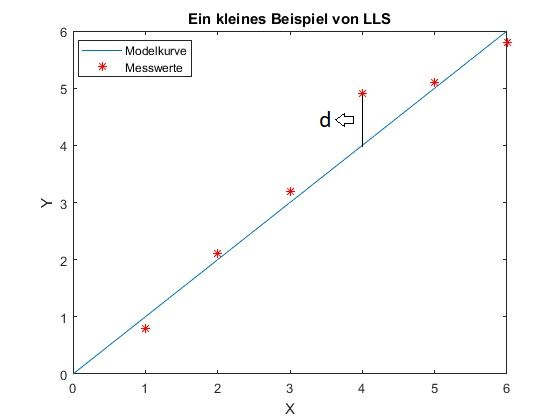
\includegraphics[scale=0.6]{img/BeispielvonLLS.jpg}
	\caption{Ein kleines Beispiel von Linear Least Square}
\end{figure}

\noindent
Das Minimum $ F(x_{i}) $ kann nur erreicht werden, wenn alle partiellen Ableitungen von F nach x null ergeben. Hier ist es zu beachten, dass Backslash-Operator rechtes Division bedeutet.

\begin{align}
\begin{split}
\frac{\delta F}{\delta \vec{x}} = 2 \cdot \underline{A}^{T} \cdot A \cdot \vec{x}-2 \cdot \underline{A}^{T} \cdot \vec{b} = 0 
\quad \Rightarrow  \quad
\vec{x}= \underline{A}^{T} \cdot A \backslash \underline{A}^{T} \cdot \vec{b}
\end{split}
\end{align}




\subsection{Mathematische Ausführung von Least Median Square }
Der Algorithmus Least Median Square (Abk. LMS) basiert auf Median und LLS. Der Median (auch Zentralwert genannt) ist der Wert in der Mitte einer der Größe nach geordneten Datenreihe. Das heißt, mindestens 50\% der Daten sind kleiner als der Median oder gleich dem Median und mindestens 50\% der Daten sind größer als der Median oder gleich dem Median(vgl. Abb.4). Bei einer ungeraden Anzahl an Datenwerten ist der Median der Wert in der Mitte. Bei einer geraden Anzahl an Datenwerten entspricht der Median dem Durchschnitt der beiden mittleren Werte. Im Vergleich zum Mittelwert ist der Median unempfindlich gegenüber Extremwerten.
\begin{figure}[H]
	\centering
	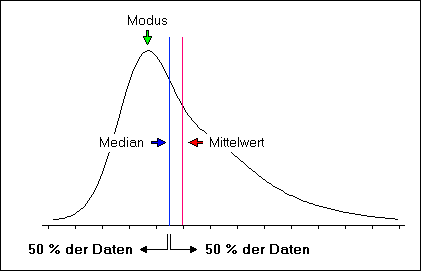
\includegraphics[scale=0.6]{img/Medianwert.png}\\
	\caption{Unterschied zwischen Median und Mittelwert}
\end{figure}
\noindent
LMS ist für das Problem wirksam, wenn fehlerbehaftete Distanzmessungen bei mehr als vier Referenzpunkte vorhanden sind. Zunächst werden alle Kombinationen mit vier zugehörigen Referenzpunkten herstellt. Wenn es beispielsweise 6 Referenzpunkte P\textsubscript{1} bis P\textsubscript{6} mit den Distanzmessungen R\textsubscript{1} bis R\textsubscript{6} gibt, dann entstehen insgesamt $(^6_4) = 15$ mögliche Subsets. Andere Möglichkeiten $(^6_5)$ und $(^6_6)$ werden hier nicht berücksichtigt, weil es für die gesucht Position P\textsubscript{lat} mit 15 Subsets reicht.
Danach wird P\textsubscript{lat} einer Kombination jeweils mit LLS-Verfahren berechnet. Hier werden insgesamt 15 berechnete Positionen mit P\textsubscript{lat(1)} bis P\textsubscript{lat(15)} hervorgebracht. Jede Position P\textsubscript{lat(k)} hat eigene Medianwert med($\vec{v}$)\textsubscript{k}. $\vec{v}$ kann mit der Abstandformel bestimmt werden.
\begin{align}
\vec{v}_{j}=|\sqrt{(X_{i}-X)^2+(Y_{i}-Y)^2+(Z_{i}-Z)^2}-R_{i}|,
\quad j \in[1,4] \,i\in[1,n]
\end{align}
X\textsubscript{i}, Y\textsubscript{i}, Z\textsubscript{i} = Koordinaten von vier Referenzpunkte einer Kombination
\newline
X, Y, Z = Koordinaten der mittels LLS berechneten P\textsubscript{lat(k)}
\newline
R\textsubscript{i} = Distanzmessung zum entsprechenden Referenzpunkt
\newline
\newline
Der Medianwert med($\vec{v}$)\textsubscript{k} von P\textsubscript{lat(k)} einer Kombination kann wie folgt ausgeführt werden:
\begin{align}
med(\vec{v})_k = median\{\vec{v}^2_1,\, \vec{v}^2_2,\, \vec{v}^2_3, \, \vec{v}^2_4\}, \quad k \in[1,(^{n}_{4})]\
\end{align}



%\cleardoublepage
\section{Ausführung in Matlab}

\subsection{LLS-Realisierung in MATLAB}
P\textsubscript{1} bis P\textsubscript{5} sind die Referenzpunkte mit den Koordinaten (X\textsubscript{1}, Y\textsubscript{1}, Z\textsubscript{1}) bis (X\textsubscript{5}, Y\textsubscript{5}, Z\textsubscript{5}) und R\textsubscript{1} bis R\textsubscript{5} die gemessene Distanzen. Folgende Referenzpunkte und Distanzmessungen sind gegeben (Einheit: Meter):
\begin{flushleft}
	P\textsubscript{1} = (10, 0, 0), R\textsubscript{1} = 10.02;\\
	P\textsubscript{2} = (0, 10, 0), R\textsubscript{2} = 10.05;\\
	P\textsubscript{3} = (0, 0, 10), R\textsubscript{3} = 9.98;\\
	P\textsubscript{4} = (-10, 0, 0), R\textsubscript{4} = 10.07;\\
	P\textsubscript{5} = (0, -10, 0), R\textsubscript{5} = 9.99;
\end{flushleft}

In MATLAB werden zuerst obige Koordinaten und Distanzen eingegeben und das lineare Gleichungssystem (3) erstellt. Danach wird die gesuchte Position P\textsubscript{lat} mit den Formeln (4) und (5)  bestimmt. Das errechnetes Ergebnis lautet  X = 0.0168, Y = -0.0301 und Z = 0.0568. Die Wahre Position ist P\textsubscript{wahr} = (0.00, 0.00, 0.00). Das Ergebnis ist sehr zufriedenstellend, obwohl es kleine Abweichungen bei praktischen Distanzmessungen gibt. Vorher wurde bereits angesprochen, dass das Ergebnis schlecht berechnet werden kann wenn eine Distanzmessung stark von der wahren Distanz abweicht. Die Distanz von R\textsubscript{1} = 15.02 ist aufgrund von NLOS-Messung, so ist die gesuchte Position P\textsubscript{lat} = (-4.16, -0.03, 2.14) (vgl. Abb.3). Das Ergebnis weicht stark von P\textsubscript{wahr} = (0.00, 0.00, 0.00) ab. Um solche fehlerbehaftete Distanzmessungen zu filtern, ist Least Median Square sinnvoll.
\begin{figure}[H]
	\centering
	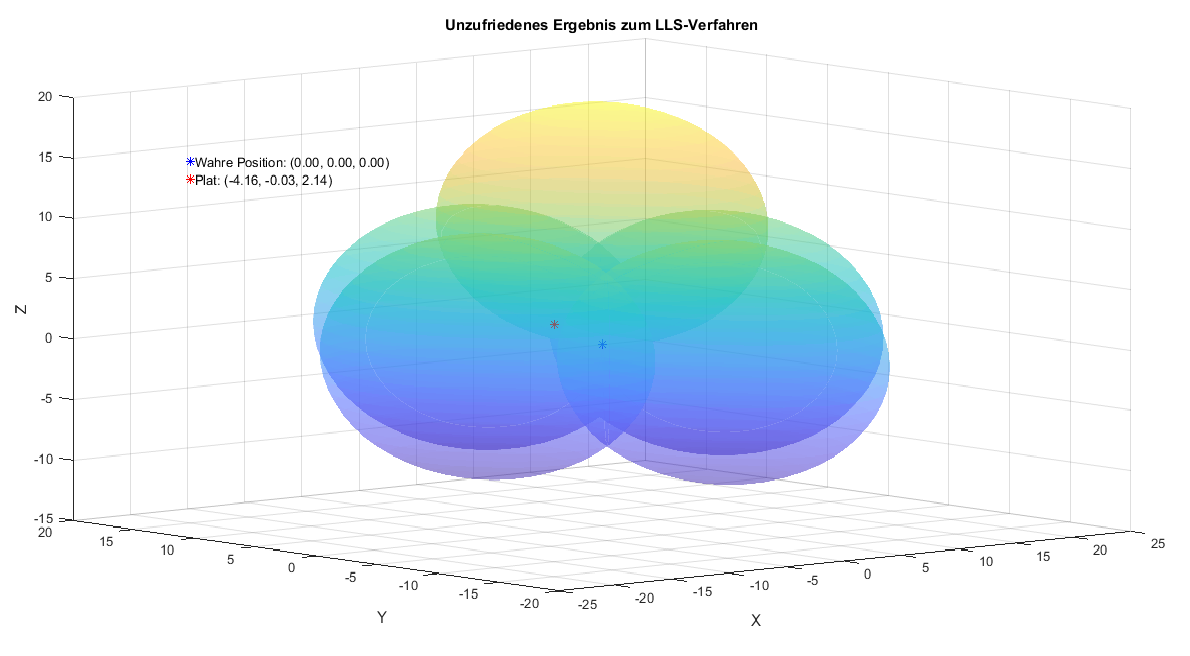
\includegraphics[scale=0.32]{img/Unzufriedenes_Ergebnis_zum_LLS-Verfahren.png}\\
	\caption{Unzufriedenes Ergebnis zum LLS-Verfahren }
\end{figure}

\subsection{LMS-Realisierung in MATLAB }
Mit den Formeln (6) und (7) kann die gesucht Position gefunden werden, die geringsten Medianwert hat. Damit können die fehlerbehaftete Distanzmessungen wegen NLOS-Messungen gefiltert werden. Jetzt ist ein Beispiel mit 6 Referenzpunkte gegeben. Alle Daten sind wie folgt dargestellt (Einheit: Meter): 
\begin{flushleft}
	P\textsubscript{1} = (10.00, 0.01, -0.01), R\textsubscript{1} = 10.20;\\
	P\textsubscript{2} = (0.02, 9.98, 0.01), R\textsubscript{2} = 9.88;\\
	P\textsubscript{3} = (0.01, 0.02, 9.56), R\textsubscript{3} = 9.54;\\
	P\textsubscript{4} = (-9.97, 0.02, 0.01), R\textsubscript{4} = 9.96;\\
	P\textsubscript{5} = (0.01, -10.01, 0.02 ), R\textsubscript{5} = 10.01;\\
	P\textsubscript{6} = (0.01, 0.03, -10.01), R\textsubscript{6} = 12.10;
\end{flushleft}
Es ist offensichtlich, dass die Distanzmessung R\textsubscript{6} zum Referenzpunkt P\textsubscript{6} durch NLOS-Messung von der wahren Distanz stark abgewichen ist und andere Distanzmessungen sehr gut sind. Hier ist die Wahre Position wieder P\textsubscript{wahr} = (0.00, 0.00, 0.00). 

In MATLAB werden zunächst die $(^6_4) = 15$ mögliche Kombinationen (\textit{Subsets}) verteilt, die von (P\textsubscript{1}, P\textsubscript{2}, P\textsubscript{3}, P\textsubscript{4}) bis (P\textsubscript{3}, P\textsubscript{4}, P\textsubscript{5}, P\textsubscript{6}) sind. Anschließend Position P\textsubscript{lat(k)} für jede Kombination mittels LLS-Verfahren ermittelt wird. Die gesuchte Postionen P\textsubscript{lat(1)} bis P\textsubscript{lat(15)} werden in MATLAB wie folgt ermittelt (Einheit: Meter):
\begin{flushleft}
P\textsubscript{lat(1)}: (-0.1059, 0.1959, 0.1202);\\
P\textsubscript{lat(2)}: (-0.2522, 0.0498, -0.0323);\\
P\textsubscript{lat(3)}: (0.9208,  1.2216, 1.1910);\\
P\textsubscript{lat(4)}: (-0.0086, 0.0984, 97.3134);\\
P\textsubscript{lat(5)}: (-0.1038, 0.1938, 2.2126);\\
P\textsubscript{lat(6)}: (-0.2463, 0.0510, 2.3456);\\
P\textsubscript{lat(7)}: (-0.1061, -0.0955, 0.1024);\\
P\textsubscript{lat(8)}: (-0.6238, -1035.1, 0.6615);\\
P\textsubscript{lat(9)}: (0.9176, -1.1126, 1.1898);\\
P\textsubscript{lat(10)}: (-0.1040,-0.0913, 2.2121);\\
P\textsubscript{lat(11)}: (0.0399, 0.0496, -0.0322);\\
P\textsubscript{lat(12)}: (-1.1305, 1.2236, 1.1910);\\
P\textsubscript{lat(13)}: (2324.7, -1.1126, 1.1898);\\
P\textsubscript{lat(14)}: (0.0387, 0.0508, 2.3544);\\
P\textsubscript{lat(15)}: (-1.1294,-1,.1126 1.1898);
\end{flushleft}

\noindent
Mittels Formel (6) \& (7) können die Medianwerte von med($\vec{v}$)\textsubscript{1} bis med($\vec{v}$)\textsubscript{15} für jede Position P\textsubscript{lat(k)} ermittelt werden. In MATLAB ergeben sich folgende Medianwerte:
\begin{flushleft}
med($\vec{v}$)\textsubscript{1} = 0,0088 $m^2$\\
med($\vec{v}$)\textsubscript{2} = 0,0028 $m^2$\\
med($\vec{v}$)\textsubscript{3} = 0,9591 $m^2$\\
med($\vec{v}$)\textsubscript{4} = 7714,0 $m^2$\\
med($\vec{v}$)\textsubscript{5} = 0,0221 $m^2$\\
med($\vec{v}$)\textsubscript{6} = 0,1015 $m^2$\\
med($\vec{v}$)\textsubscript{7} = 0,0089 $m^2$\\
med($\vec{v}$)\textsubscript{8} = 105077 $m^2$\\
med($\vec{v}$)\textsubscript{9} = 0,9607 $m^2$\\
med($\vec{v}$)\textsubscript{10} = 0,0217 $m^2$\\
med($\vec{v}$)\textsubscript{11} = 0,0025 $m^2$\\
med($\vec{v}$)\textsubscript{12} = 0,9321 $m^2$\\
med($\vec{v}$)\textsubscript{13} = 535792 $m^2$\\
med($\vec{v}$)\textsubscript{14} = 0,1017 $m^2$\\
med($\vec{v}$)\textsubscript{15} = 0,9345 $m^2$
\end{flushleft}
\noindent
Um bessere Visualisierung zu erreichen, werden die Medianwerte in Balkendiagramm dargestellt.
\begin{figure}[H]
	\centering
	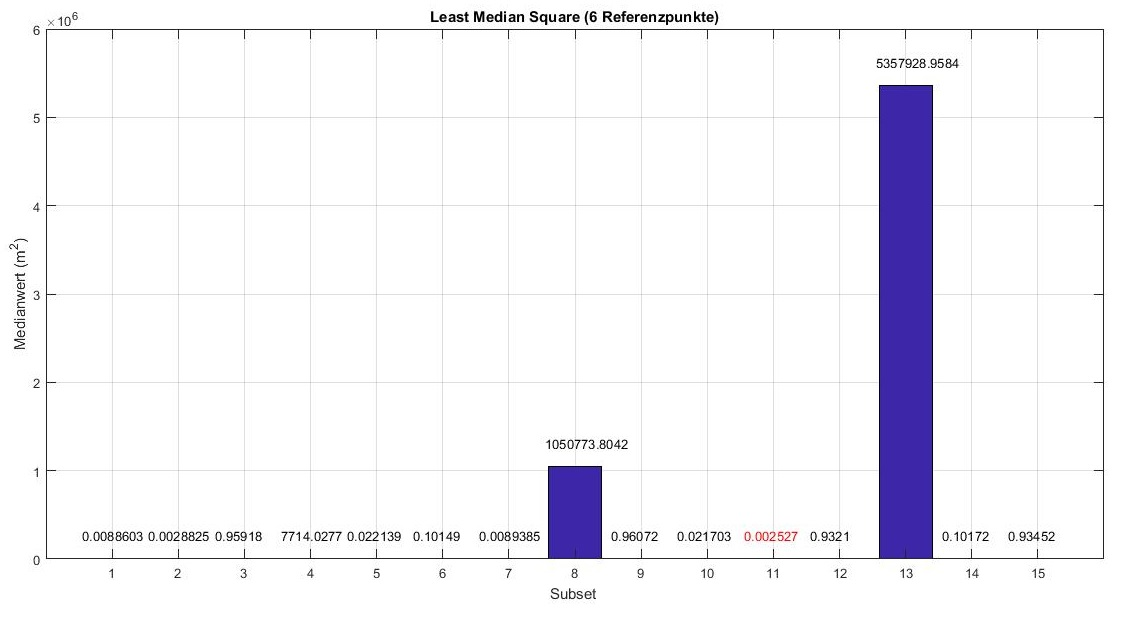
\includegraphics[scale=0.40]{img/LMS_Medianwert.jpg}\\
	\caption{Medianwert med($\vec{v}$)\textsubscript{k} bei LMS-Verfahren }
\end{figure}

\noindent
 Mit diesem Balkendiagramm ist es offensichtlich zu sehen, dass med($\vec{v}$)\textsubscript{11} den geringsten Medianwert bekommt. Die Kombination(\textit{Subset}) der optimierten Referenzpunkte sind P\textsubscript{2}, P\textsubscript{3}, P\textsubscript{4} und P\textsubscript{5}. P\textsubscript{6} mit offensichtlicher NLOS-Messung R\textsubscript{6} und P\textsubscript{1} mit kleinem Messfehler R\textsubscript{1} werden erfolgreich gefiltert. Die gesuchte Postion ist P\textsubscript{lat(11)} = (0.0399, 0.0496, -0.0322). Die gesuchte Position und optimierte Referenzpunkte werden im 3D-Umgebung angezeigt.
\begin{figure}[H]
	\centering
	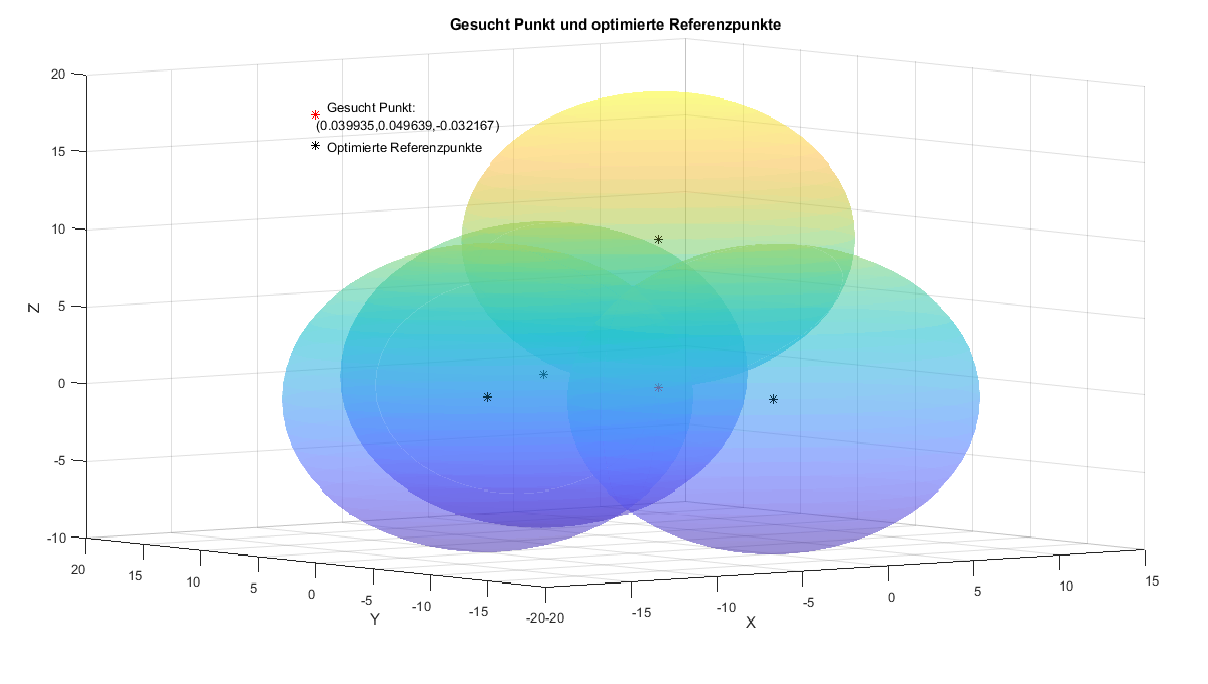
\includegraphics[scale=0.35]{img/LMS_Plat.png}\\
	\caption{Die gesucht P\textsubscript{lat(11)} und optimierte Referenzpunkte}
\end{figure}




%\cleardoublepage
\section{Zusammenfassung und Ausblick}
Wenn keine Messfehler vorhanden sind, ist Least Linear Square ein direktester Algorithmus zur Lokalisierung einer Position. LLS unterstützt selbst nicht, um die berechnete Ergebnisse zu vergleichen und die Messfehler zu filtern. Im Vergleich zur LLS kann Least Median Square das optimiertes Ergebnisses mit dem Medianwert finden, um die Genauigkeit einer Position zu erhöhen.\\
Der Kern von LMS ist die Verwendung des Medianwertes, aber der Medianwerte spielt leid nicht immer beste Rolle in allen Fällen. Der Medianwert funktioniert gut, wenn es nur ein paar offensichtliche Messfehler vorhanden gibt. Falls alle Messungen genau oder wenig abwicht, spiele der Mittelwert theoretisch besser als Medianwert. Nach vielen Testen von MATLAB zeigt Mittelwert aber gar keinen Vorteil. Solche Testdaten entsprechen aber nicht der Theorie. Es ist notwendig, um das Problem weiter zu löschen, aber in diese Projektarbeit wird es nicht mehr geforscht.

%\cleardoublepage
\section{MATLAB Code}
MATLAB Code besteht aus 2 Teile. 
Der erste Teil realisiert die Funktion von das Least Median Square, die LMS-Algorithmus ausführt.
Der zweite Teil ist Script von Least Median Square, die durch den Aufruf der LMS-Funktion notwendige Ergebnisse erhalten kann, damit werden alle Medianwerte med($\vec{v}$)\textsubscript{1} bis med($\vec{v}$)\textsubscript{n} mit dem Balkendiagramm und gesuchte Position P\textsubscript{lat(i)} \& optimierte Referenzpunkte mit dem 3D-Diagramm darstellt.

\subsection{Funktion von Least Median Square}
\lstinputlisting{LMS2_Funk.m}
\subsection{Script von Least Median Square}
\lstinputlisting{LMS2_Script.m} 

%\cleardoublepage
%\include{listsend} %enthaelt Literatur-, Abbildungs- und Tabellenverzeichnis

\end{document}
%
% end of document
         % the index has to be generated manually by an extra tool
%
%
\chapter*{The author}
%
\label{sec:TheAuthor}%
\addcontentsline{toc}{section}{The Author}
%
\begin{figure}[h]
\begin{flushright}
%\begin{center}
	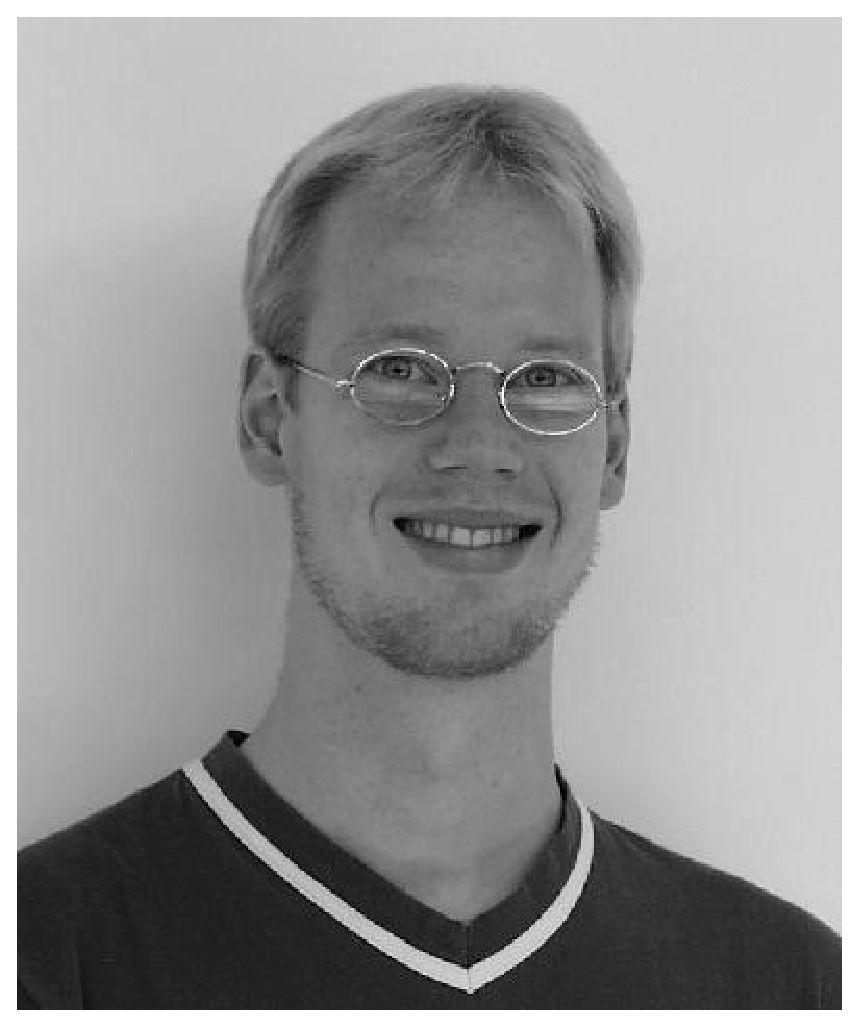
\includegraphics[width =0.2\textwidth]{img/koch}
%\end{center}
\end{flushright}
\end{figure}
%
%
Carsten Koch was born in 1974 in L\"{u}neburg,
Germany. From 1994 to 1999 he studied at the University of Applied
Sciences in L\"{u}neburg, and he holds a degree in Automation and
Electronics.

After his graduation he enrolled in City University, London, in
the department of Electrical, Electronic and Information
Engineering as a research student. The research was supervised by
Prof.~T.J.~Ellis.%, who was leading the Machine Vision Group at
%City University until .

In 1999 he joined the BMW research and development department in
Munich, Germany, where most of this research was performed.

Today the author and his family live in northern Germany, where he
founded a consulting company for image sensors in 2002. He teaches
courses in digital electronics at the Leuphana University L\"{u}neburg.




%\addcontentsline{toc}{section}{Hallo}

\end{document}
%
% end of document
